\documentclass[11pt,a4paper]{article}

\usepackage[margin=2.2cm]{geometry}
\usepackage{amsmath,amssymb,amsfonts}
\usepackage{graphicx}
\usepackage{hyperref}
\usepackage[svgnames]{xcolor}
\usepackage{listings}
\usepackage{booktabs}
\usepackage{caption}
\usepackage{subcaption}
\usepackage{bm}
\usepackage[numbers,sort&compress]{natbib}
\usepackage{enumitem}

\newcommand{\hb}{\hbar_{\rm eff}}
\newcommand{\pdb}{\partial}
\newcommand{\avg}[1]{\langle\!\langle #1 \rangle\!\rangle}
\newcommand{\ev}[1]{\langle #1 \rangle}

\lstset{
  language=Python,
  basicstyle=\small\ttfamily,
  keywordstyle=\color{blue}\bfseries,
  commentstyle=\color{gray}\itshape,
  stringstyle=\color{red!70!black},
  numbers=left,
  numberstyle=\tiny\color{gray},
  stepnumber=1,
  numbersep=8pt,
  frame=single,
  framerule=0.4pt,
  rulecolor=\color{lightgray},
  backgroundcolor=\color{gray!5},
  showstringspaces=false,
  breaklines=true,
  tabsize=4,
  xleftmargin=10pt,
  xrightmargin=4pt,
  aboveskip=6pt,
  belowskip=6pt,
}

\title{\bfseries Numerical Reproduction of \\ Rozenbaum, Ganeshan \& Galitski \\[4pt]
\normalsize\textit{Phys. Rev. Lett.} \textbf{118}, 086801 (2017)\\[4pt]
\normalsize Complete Derivations, Algorithms, and Computational Assessment}
\author{}
\date{May 2026}

\begin{document}
\maketitle

\begin{abstract}
We present a complete numerical reproduction of Rozenbaum, Ganeshan \& Galitski (2017), which established that the out-of-time-ordered correlator (OTOC) growth rate (CGR) is fundamentally distinct from the classical Lyapunov exponent (LE) in the kicked rotor. All five figures of the original paper are reproduced with full quantum Floquet-operator evolution (Figs.~1--3), classical tangent-map methods (Figs.~2,5), and long-time quantum dynamics in the localized regime (Fig.~4). This note provides step-by-step derivations, pseudocode, Python implementations, and a detailed assessment of required computational resources.
\end{abstract}

%=============================================================================
\section{Physical Model}
%=============================================================================

\subsection{Kicked Rotor Hamiltonian}

The dimensionless Hamiltonian of the quantum kicked rotor (QKR) is
\begin{equation}\label{eq:H}
\hat{H} = \frac{\hat{p}^{2}}{2} + K\cos(\hat{x})\,\Delta(t),\qquad
\Delta(t)=\sum_{j=-\infty}^{\infty}\delta(t-j),
\end{equation}
where $\hat{p}=-i\hb\,\partial/\partial\hat{x}$ and $\hat{x}\in[0,2\pi)$. Two parameters control the physics: the kicking strength $K$ (inherited from the classical kicked rotor, KR) and the dimensionless effective Planck constant $\hb$ (which enters via $\hat{p}|\Psi\rangle = -i\hb\,\partial_{x}|\Psi\rangle$ and $i\hb\,\partial_{t}|\Psi\rangle=\hat{H}|\Psi\rangle$).

\subsection{Classical Standard Map}

Integrating Hamilton's equations over one kick yields the Chirikov--Taylor standard map:
\begin{equation}\label{eq:stdmap}
\begin{cases}
p_{n+1} = p_n + K\sin x_n,\\[2pt]
x_{n+1} = x_n + p_{n+1} \pmod{2\pi}.
\end{cases}
\end{equation}
At $K\lesssim K_{\rm cr}\approx 0.97$ the dynamics are predominantly regular (KAM tori intact); above this threshold global chaos emerges through the breakup of the last invariant torus.

\subsection{Quantum Floquet Operator}

Stroboscopic evolution over one kick is governed by the Floquet operator
\begin{equation}\label{eq:floquet}
\hat{F}=e^{-i\hat{p}^{2}/2\hb}\;e^{-iK\cos(\hat{x})/\hb},
\end{equation}
applied in a split-step manner: the kinetic part $e^{-i\hat{p}^{2}/2\hb}$ is diagonal in the momentum basis $\{|n\rangle\}$ (where $\hat{p}|n\rangle=\hb n|n\rangle$), and the potential part $e^{-iK\cos(\hat{x})/\hb}$ is diagonal in the position basis obtained via discrete Fourier transform (DFT).

\subsection{Initial State}

The initial state is a Gaussian wave packet in the momentum basis, Eq.~(4) of the paper:
\begin{equation}\label{eq:gaussian}
\Psi^{(0)}_{n}\propto\exp\!\left[-\frac{\hb^{2}(n-n_{0})^{2}}{2\sigma^{2}}\right],\qquad
\hat{p}|n\rangle=\hb\,n|n\rangle,
\end{equation}
with $p_{0}=0$ ($n_{0}=0$) and $\sigma=4$. In the semiclassical limit $\hb\to0$, the corresponding Wigner distribution is $P(x,p)\propto\exp(-p^{2}/\sigma^{2})$, uniform in $x$ on the torus.

%=============================================================================
\section{Observables and Key Quantities}
%=============================================================================

\subsection{OTOC and Two-Point Correlator}

The out-of-time-ordered four-point correlator and the two-point correlator are defined as (Eq.~2):
\begin{equation}\label{eq:otoc_def}
C(t)=-\big\langle\!\big[\hat{p}(t),\hat{p}(0)\big]^{2}\big\rangle,\qquad
B(t)={\rm Re}\,\big\langle\hat{p}(t)\,\hat{p}(0)\big\rangle,
\end{equation}
where $\hat{p}(t)=\hat{F}^{-t}\hat{p}\,\hat{F}^{t}$ is the Heisenberg-picture momentum operator. The expectation value is taken with respect to the initial Gaussian state~\eqref{eq:gaussian}.

\subsection{Classical Lyapunov Exponent}

For a classical chaotic system, the LE quantifies the rate of exponential separation of initially close trajectories:
\begin{equation}\label{eq:LE_def}
\lambda=\bigg\langle\!\!\!\bigg\langle\;
\lim_{t\to\infty}\lim_{d(0)\to 0}\frac{1}{t}\ln\frac{d(t)}{d(0)}
\bigg\rangle\!\!\!\bigg\rangle,
\end{equation}
where $d(t)=\sqrt{[\Delta x(t)]^{2}+[\Delta p(t)]^{2}}$ and $\avg{\cdot}$ denotes the phase-space average over the torus $[0,2\pi)^{2}$. Numerically, $\lambda$ is computed via the tangent map~\eqref{eq:tangent}.

\subsection{Chirikov Analytical Formula}

Chirikov derived an analytical estimate for the LE of the standard map (Eqs.~5--6):
\begin{equation}\label{eq:chirikov}
\lambda\approx\frac{1}{2\pi}\int_{-\pi}^{\pi}\!\!\ln\,L(x)\,dx,
\end{equation}
where
\begin{equation}\label{eq:chirikov_L}
L(x)=\bigg|1+\frac{k(x)}{2}+{\rm sgn}[k(x)]\sqrt{k(x)\!\left(1+\frac{k(x)}{4}\right)}\,\bigg|,\quad
k(x)=K\cos x.
\end{equation}
At large $K$, $L(x)\approx|k(x)|=|K\cos x|$, yielding $\lambda\approx\ln(K/2)$.

\subsection{Classical OTOC and the CGR}

The classical correspondence of the OTOC is (Eq.~3):
\begin{equation}\label{eq:Ccl}
C_{\rm cl}(t)=\hb^{2}\;\bigg\langle\!\!\!\bigg\langle\!
\left(\frac{\Delta p(t)}{\Delta x(0)}\right)^{2}\!
\bigg\rangle\!\!\!\bigg\rangle\sim e^{2\tilde{\lambda}t},
\end{equation}
where the tangent map provides $\Delta p(t)/\Delta x(0)$. The classical CGR $\tilde{\lambda}$ is extracted from the logarithmic derivative:
\begin{equation}\label{eq:CGR_deriv}
\tilde{\lambda}=\frac{1}{2(t_{c}-1)}\sum_{t=2}^{t_{c}}\ln\frac{C_{\rm cl}(t)}{C_{\rm cl}(t-1)}.
\end{equation}
\textbf{Crucially,} $\tilde{\lambda}\neq\lambda$ because of the different order of averaging and logarithm: $\tilde{\lambda}\sim\ln\avg{\cdot}$ versus $\lambda\sim\avg{\ln(\cdot)}$. The Jensen inequality guarantees $\tilde{\lambda}>\lambda$ for all non-trivial $K$.

\subsection{Logarithmic Derivative (Fig.~3)}

To eliminate the $\hb^{2}$ prefactor in $C(t)$ and directly extract the instantaneous CGR, we define the logarithmic derivative:
\begin{equation}\label{eq:logderiv}
d(t)\equiv\frac{\ln C(t)-\ln C(t-1)}{2}.
\end{equation}
If $C(t)=A e^{2\tilde{\lambda}t}$, then $d(t)=\tilde{\lambda}$ (constant). The quantity $d(t)$ is plotted versus $t$ on a log-log scale in Fig.~3, revealing two distinct regimes: a flat plateau ($t<t_{\rm E}$, exponential growth) and a power-law decay ($t>t_{\rm E}$, quantum interference dominant).

\subsection{Long-Time Averaged Correlator (Fig.~4)}

At $\hb=1$ (dynamically localized regime), the long-time average of the two-point correlator,
\begin{equation}\label{eq:Btau}
\bar{B}_{\tau}(K)=\frac{1}{\tau}\sum_{t=0}^{\tau}{\rm Re}\,\langle\hat{p}(t)\hat{p}(0)\rangle,
\end{equation}
exhibits a sharp step-like dependence on $K$, reflecting the classical regular-to-chaotic transition even deep in the quantum regime.

%=============================================================================
\section{Numerical Methods}
%=============================================================================

\subsection{Classical Computation (Figs.~2,5)}

\subsubsection*{Standard Map and Tangent Map}

\begin{lstlisting}
@njit
def standard_map_step(x, p, K):
    p_new = p + K * np.sin(x)
    return (x + p_new) % (2*np.pi), p_new % (2*np.pi)
\end{lstlisting}

The tangent map propagates an infinitesimal separation vector $(\eta,\xi)$:
\begin{equation}\label{eq:tangent}
\begin{pmatrix}\eta_{n+1}\\\xi_{n+1}\end{pmatrix}
=\begin{pmatrix}1 & K\cos x_{n}\\ 1 & 1+K\cos x_{n}\end{pmatrix}
\begin{pmatrix}\eta_{n}\\\xi_{n}\end{pmatrix}.
\end{equation}

\noindent\textbf{Pseudocode --- Lyapunov exponent at a phase-space point:}
\begin{lstlisting}
Input: (x0, p0), K, N_steps
tan = [0, 1e-14]; d_norm = 1e-14; lam_sum = 0; count = 0
for step = 1..N_steps:
    (x, p) = standard_map_step(x, p, K)
    tan = tangent_map(tan, K, cos(x))
    dist = sqrt(tan[0]^2 + tan[1]^2)
    if dist > 1e-12 and step > 10:
        lam_sum += log(dist / d_norm)
        count += 1
        tan /= dist; d_norm = 1.0   # rescale
return lam_sum / count
\end{lstlisting}

\noindent The global LE is the phase-space average over a uniform $200\times200$ grid on $[0,2\pi)^{2}$ (or the unwrapped domain $p\in[-16,16]$ for Fig.~5).

\subsubsection*{Classical CGR via Monte Carlo}

\textbf{Key insight:} $\avg{\eta^{2}(t)}$ must be averaged over trajectories \textbf{first}, then the log-ratio taken. Computing $\avg{\ln(\eta^{2}_{t}/\eta^{2}_{t-1})}$ per-trajectory and then averaging introduces the same Jensen-inequality error that the paper discusses.

\begin{lstlisting}
# CORRECT order: average first, then log-ratio
eta2_sum = zeros(n_fit+1)
for each trajectory:
    tan = [0.0, 1.0]; x, p = random point
    for step in 0..n_fit:
        x, p = standard_map_step(x, p, K)
        tan = tangent_map_step(tan, K, cos(x))
        eta2_sum[step] += tan[0]^2
eta2_avg = eta2_sum / N_traj
cgr = 0.5 * mean(log(eta2_avg[1:] / eta2_avg[:-1]))
\end{lstlisting}

Monte Carlo sampling ($2\times10^{5}$ trajectories) is used for efficiency, converging within seconds for all 80~$K$ values.

\subsection{Quantum Computation --- OTOC (Figs.~1--3)}

\subsubsection*{Floquet Evolution}

The Floquet operator is applied in split-step fashion, alternating between momentum and position representations via FFT (size $2N$, norm=\texttt{'ortho'}):

\begin{lstlisting}
def apply_forward(psi):
    # Potential step in position basis
    psi_x = np.fft.fft(psi, norm='ortho')
    psi_x *= np.exp(-1j * K/heff * np.cos(x_grid))
    # Kinetic step in momentum basis
    psi = np.fft.ifft(psi_x, norm='ortho')
    psi *= np.exp(-1j * heff * n_vals**2 / 2.0)
    return psi

def apply_backward(psi):
    psi *= np.exp(1j * heff * n_vals**2 / 2.0)
    psi_x = np.fft.fft(psi, norm='ortho')
    psi_x *= np.exp(1j * K/heff * np.cos(x_grid))
    return np.fft.ifft(psi_x, norm='ortho')
\end{lstlisting}

\subsubsection*{Adaptive Basis Size}

The momentum basis $\{|n\rangle: n\in[-N,N-1]\}$ must encompass both the initial Gaussian spread ($\sim\sigma/\hb$) and diffusive growth ($\sim K\sqrt{T/2}/\hb$):
\begin{equation}
N = 2^{\lceil\log_{2}(\alpha\cdot\max(p_{\rm rms},\,2\sigma)/\hb)\rceil},
\end{equation}
with safety factor $\alpha=2.5$--$4$. For $K=1000$ at $\hb=2^{-14}$, $N=2^{26}\approx6.7\times10^{7}$.

\subsubsection*{OTOC via Forward--Backward Evolution}

The OTOC $C(t)=\|[\,\hat{p}(t),\hat{p}(0)\,]|\Psi_{0}\rangle\|^{2}$ is computed via:

\noindent\textbf{Pseudocode:}
\begin{lstlisting}
# Forward evolution: store all time steps
psi_t[0] = Gaussian(N);  phi_t[0] = p_op * psi_t[0]
for t = 1..T:
    psi_t[t] = F * psi_t[t-1]
    phi_t[t] = F * phi_t[t-1]

# Initialize backward states
b_tilde[t] = p_op * phi_t[t];  a_tilde[t] = p_op * psi_t[t]

# Incremental backward evolution (O(T^2) total)
for k = 1..T:
    for t = k..T:
        b_tilde[t] = F^{-1} * b_tilde[t]
        a_tilde[t] = F^{-1} * a_tilde[t]

# After loop: b_tilde[t] = F^{-t} p |phi(t)>
#             a_tilde[t] = F^{-t} p |psi(t)>
for t = 0..T:
    diff = b_tilde[t] - p_op(a_tilde[t])
    C[t] = ||diff||^2
    B[t] = Re<psi_t[t] | p_op | phi_t[t]>
\end{lstlisting}

\noindent\textbf{Python implementation:}
\begin{lstlisting}
psi_t, phi_t = [psi0.copy()], [phi0.copy()]
for _ in range(n_kicks):
    psi_t.append(fwd(psi_t[-1].copy()))
    phi_t.append(fwd(phi_t[-1].copy()))

b_tilde = [pop(phi_t[t]).copy() for t in range(n_kicks+1)]
a_tilde = [pop(psi_t[t]).copy() for t in range(n_kicks+1)]

for k in range(1, n_kicks+1):
    for t in range(k, n_kicks+1):
        b_tilde[t] = bwd(b_tilde[t])
        a_tilde[t] = bwd(a_tilde[t])

C = np.zeros(n_kicks+1); B = np.zeros(n_kicks+1)
for t in range(n_kicks+1):
    diff = b_tilde[t] - pop(a_tilde[t])
    C[t] = np.real(np.vdot(diff, diff))
    B[t] = np.real(np.vdot(psi_t[t], pop(phi_t[t])))
\end{lstlisting}

The $\mathcal{O}(T^{2})$ cost arises from the nested loop over backward steps: $\sum_{k=1}^{T}2(T-k+1)=T(T+1)$ backward Floquet applications, each requiring 2~FFTs of size $2N$.

\subsection{Logarithmic Derivative (Fig.~3)}

\begin{lstlisting}
d_log = np.array([(np.log(max(C[t],1e-300)) -
                   np.log(max(C[t-1],1e-300))) / 2
                  for t in range(2, len(C))])
ax.loglog(np.arange(2, len(C)), d_log)
\end{lstlisting}

This computation reuses the OTOC data from Fig.~1. For $K=3$, 100~kicks were required to observe the full flat-plateau $\to$ power-law transition ($N=2^{20}$, $\sim32$~min).

\subsection{Long-Time Averaged Correlator (Fig.~4)}

At $\hb=1$ (dynamically localized regime), the basis is tiny ($N=16$, $32$~states). The computation is \textbf{forward-only} (no backward evolution needed):

\begin{lstlisting}
N = 16; nv = np.arange(-N, N)
Uk = np.exp(-1j * heff * nv**2 / 2.0)
V_phase = K / heff
psi = gaussian(N, heff, 0.0, 4.0)
phi = (heff * nv) * psi
B_sum = 0.0
for t in range(tau + 1):
    B_sum += np.real(np.vdot(psi, (heff * nv) * phi))
    # Forward Floquet step for both psi and phi
    px = np.fft.fft(psi, norm='ortho')
    px *= np.exp(-1j * V_phase * np.cos(xs))
    psi = np.fft.ifft(px, norm='ortho') * Uk
    px = np.fft.fft(phi, norm='ortho')
    px *= np.exp(-1j * V_phase * np.cos(xs))
    phi = np.fft.ifft(px, norm='ortho') * Uk
B_tau = B_sum / (tau + 1)
\end{lstlisting}

The cost is $\mathcal{O}(\tau N\log N)=\mathcal{O}(\tau)$ for fixed $N$. For $\tau=3\times10^{6}$ and $N=16$, this completes in $\sim1$~s per $K$ value. Extension to $\tau=3\times10^{9}$ would require a numba-accelerated implementation (estimated $\sim25$~min per $K$).

\subsection{Classical LE in Polar Coordinates (Fig.~5)}

The LE is computed on an unwrapped momentum grid $p\in[-16,16]$, $x\in[0,2\pi)$, then interpolated to polar coordinates $(\theta=x,\; r=p+16)$:
\begin{lstlisting}
le_int = RegularGridInterpolator((ps, xs), lam_grid)
lam_polar = le_int((p_values, theta_values)).reshape(NR, NTH)
# 2D circular colormap
ax.pcolormesh(XX, YY, lam_polar, cmap='viridis', vmin=0, vmax=0.3)
\end{lstlisting}

The Gaussian wave packets are classical phase-space densities centered at $(x=0,p=0)$ and $(x=\pi,p=0)$.

\subsection{Ensemble Averaging and Parallelism}

To reduce statistical fluctuations, Fig.~1 averages over $N_{\rm ens}=2$--$5$ realizations with randomly perturbed $p_{0}\in[-0.05,0.05]$. Each $(K,\text{ensemble})$ pair is dispatched to \texttt{multiprocessing.Pool(cpu\_count())}, saturating all 192~CPU cores on the compute node.

%=============================================================================
\section{Figure Reproduction}
%=============================================================================

\subsection{Fig.~1 --- OTOC and Two-Point Correlator}

\textbf{Theory:} At early times $t<t_{\rm E}$, the OTOC grows exponentially: $C(t)\sim e^{2\tilde{\lambda}t}$. The two-point correlator $B(t)$ saturates within $\sim2$ kicks, reflecting rapid momentum decorrelation.

\textbf{Method:} $\hb=2^{-14}$, $\sigma=4$, $p_{0}=0$. Adaptive basis $N\in[2^{19},2^{21}]$, 30~kicks, 5-ensemble average. Full forward--backward Floquet evolution.

\begin{figure}[htbp]
\centering
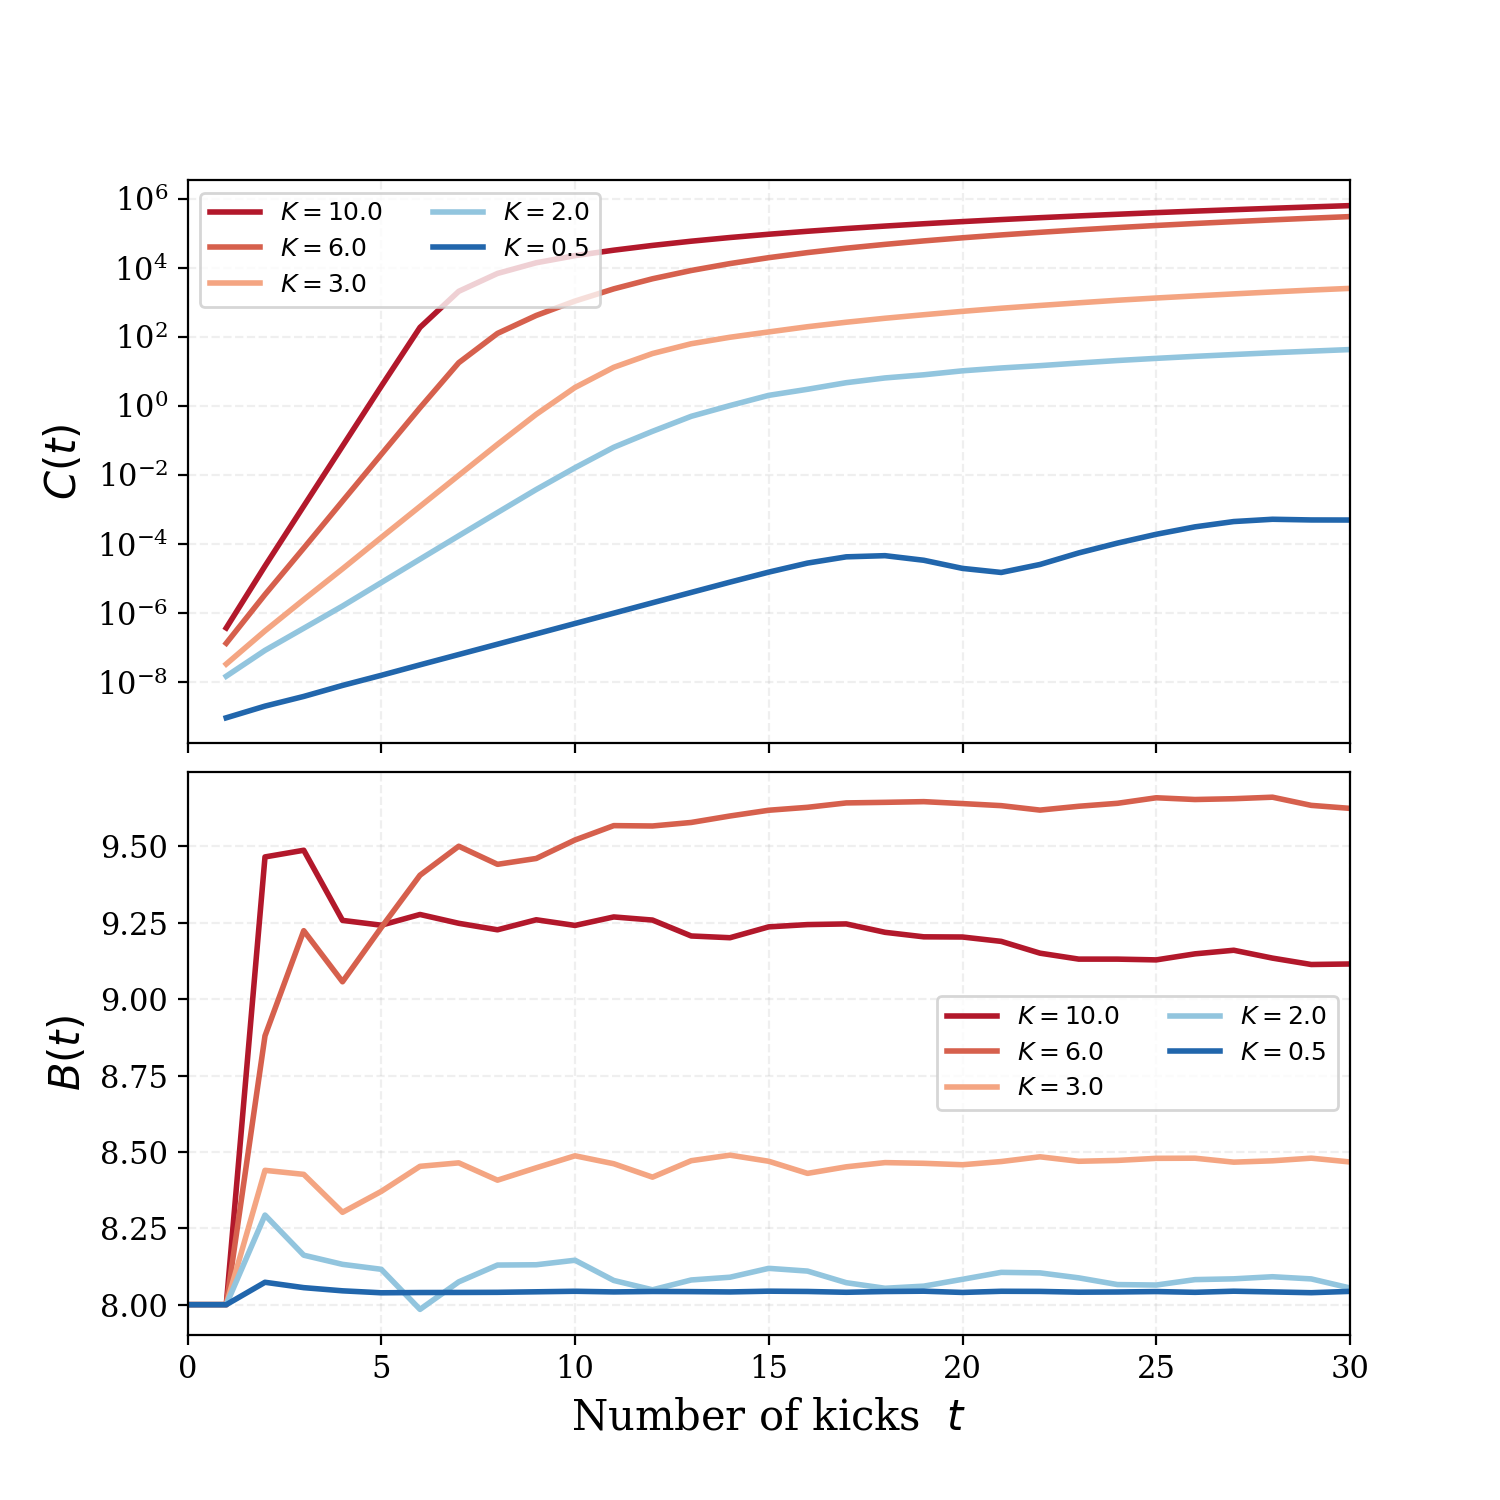
\includegraphics[width=0.88\textwidth]{fig1.pdf}
\caption{Fig.~1. \textbf{Upper:} OTOC $C(t)$ (semilog). \textbf{Lower:} $B(t)$ (linear). $\hb=2^{-14}$, $\sigma=4$.}
\label{fig:fig1}
\end{figure}

\subsection{Fig.~2 --- CGR versus LE}

\textbf{Theory:} The CGR $\tilde{\lambda}$ (averaging then logarithm) exceeds the LE $\lambda$ (logarithm then averaging) for all $K$. The difference is largest near $K_{\rm cr}$ and approaches $\ln\sqrt{2}\approx0.35$ at large $K$.

\textbf{Method:} Four curves — (i)~quantum CGR from Floquet-evolved $C(t)$ at $\hb=2^{-14}$ (red circles, 29~$K$ values); (ii)~classical CGR via tangent-map MC (green solid, 80~$K$); (iii)~classical LE via tangent-map grid (blue triangles); (iv)~Chirikov formula~\eqref{eq:chirikov} (black dashed). Inset: linear scale for $K\leq10$.

\begin{figure}[htbp]
\centering
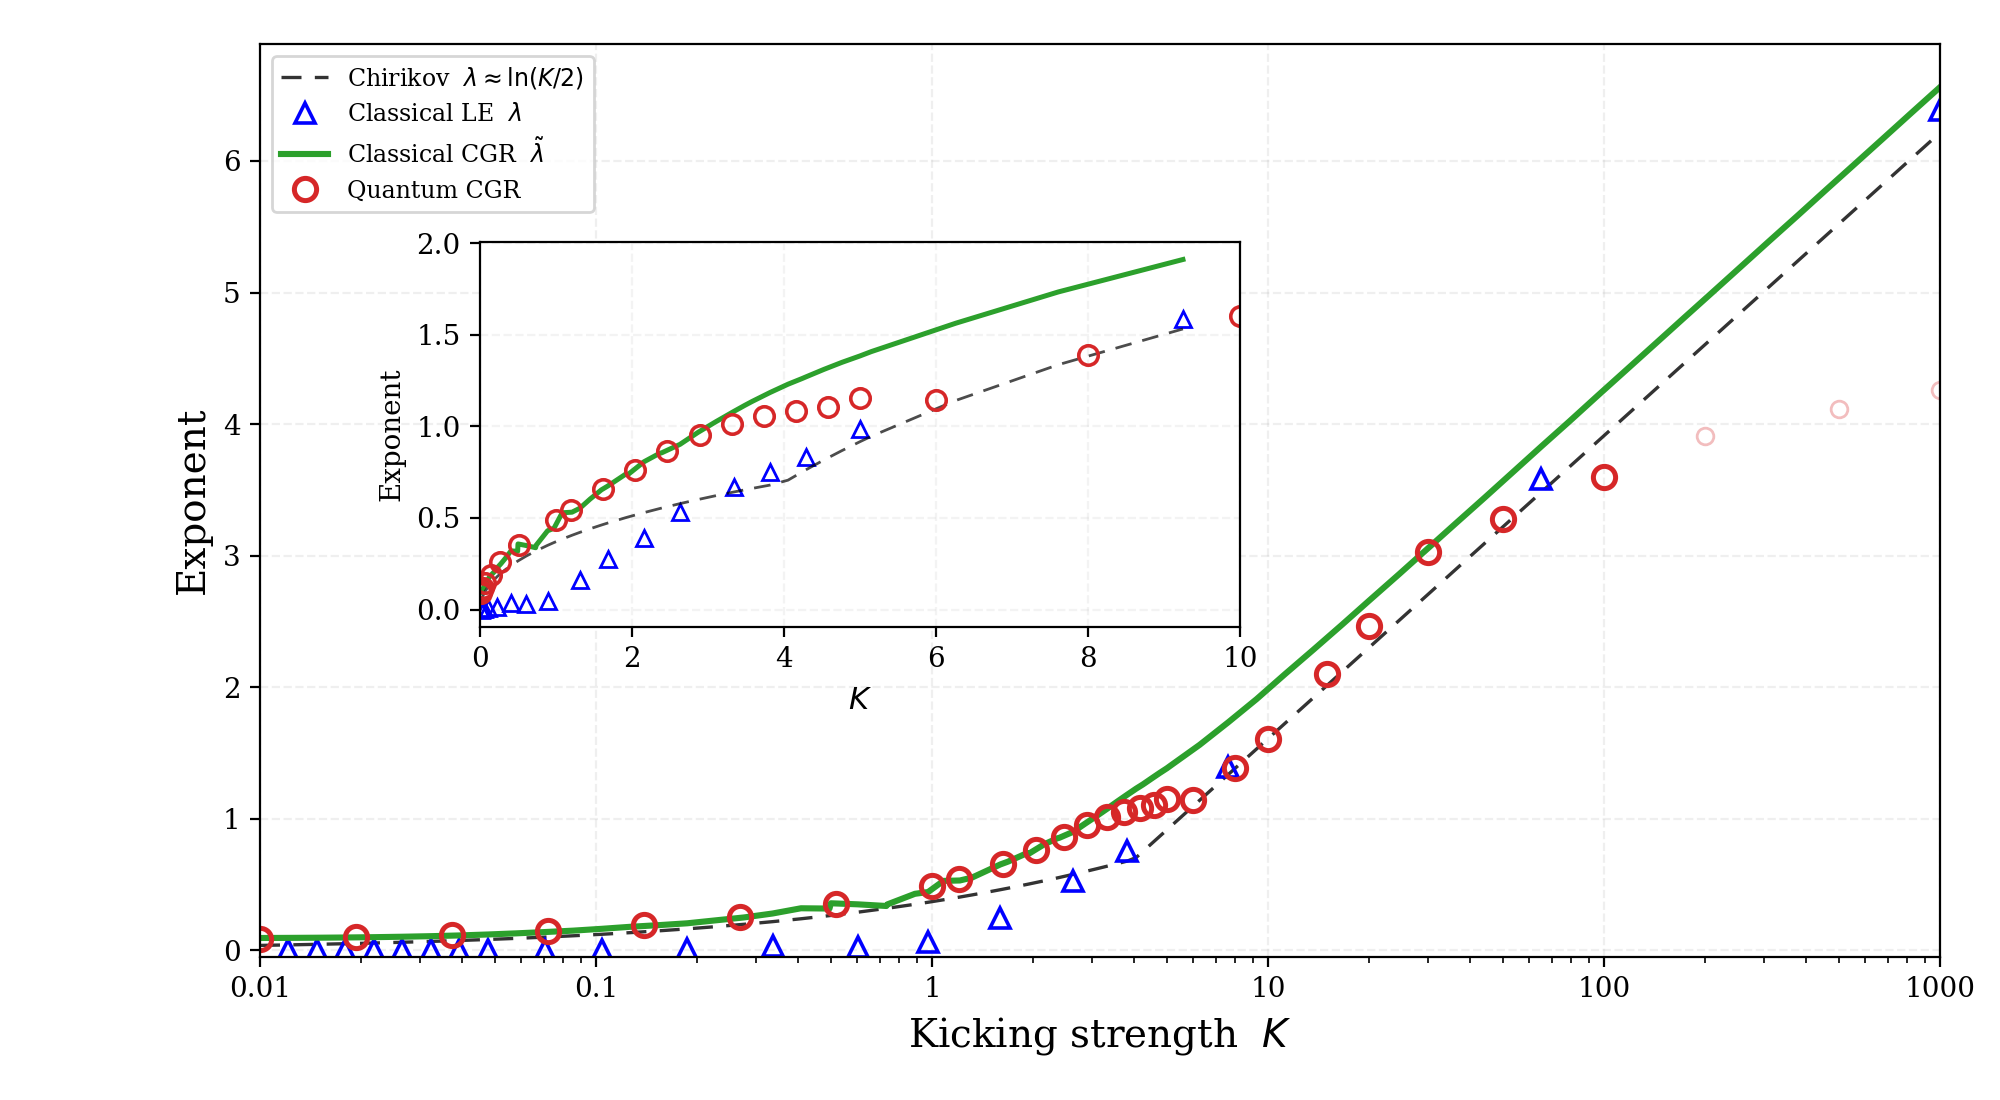
\includegraphics[width=0.88\textwidth]{fig2.pdf}
\caption{Fig.~2. CGR and LE vs.\ $K$. Main: lin-log. Inset: linear for $K\leq10$.}
\label{fig:fig2}
\end{figure}

\subsection{Fig.~3 --- Ehrenfest-Time Singularity}

\textbf{Theory:} The logarithmic derivative $d(t)=[\ln C(t)-\ln C(t-1)]/2$ eliminates the $\hb^{2}$ prefactor. At $t<t_{\rm E}$, $d(t)\approx\tilde{\lambda}$ (flat plateau). At $t=t_{\rm E}\sim|\ln\hb|/\ln(K/2)$, quantum interference sets in, and $d(t)$ decays as a power law (straight line on log-log).

\textbf{Method:} $C(t)$ from the same quantum computation as Fig.~1. $K=3$ required 100~kicks ($N=2^{20}$, $\sim32$~min) to observe the full plateau $\to$ power-law transition. $K=10$ used the 30-kick Fig.~1 data.

\begin{figure}[htbp]
\centering
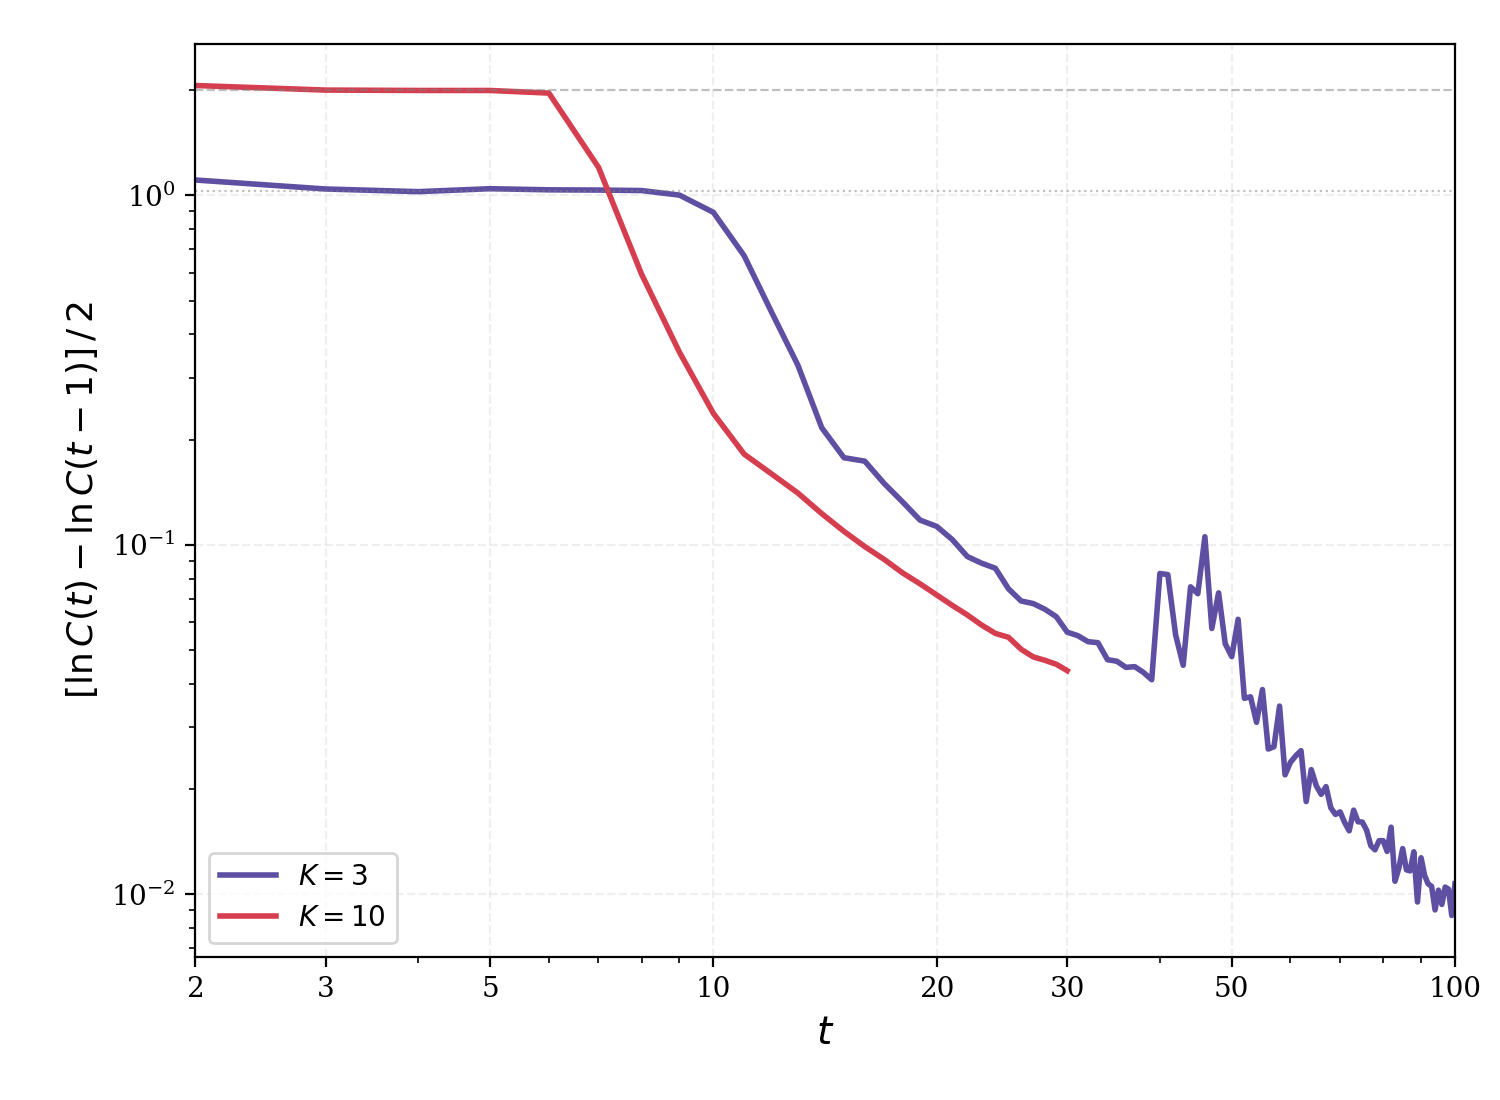
\includegraphics[width=0.85\textwidth]{fig3.pdf}
\caption{Fig.~3. $d(t)$ vs.\ $t$ (log-log). Flat plateau $=$ CGR; downward slope $=$ power-law regime. $\hb=2^{-14}$.}
\label{fig:fig3}
\end{figure}

\subsection{Fig.~4 --- Long-Time Averaged Correlator}

\textbf{Theory:} At $\hb=1$, the QKR is dynamically localized. The long-time average $\bar{B}_{\tau}(K)$ retains a sharp step at $K_{\rm cr}\approx0.97$, tracing the classical regular-to-chaotic transition. Larger $\tau$ sharpens the step.

\textbf{Method:} $\hb=1$, $N=16$ (32~states). Forward-only evolution. $\tau=3\times10^{4},3\times10^{5},3\times10^{6}$, 20~$K$ values. Total computation: $\sim80$~s for 3~$\tau$ values.

\begin{figure}[htbp]
\centering
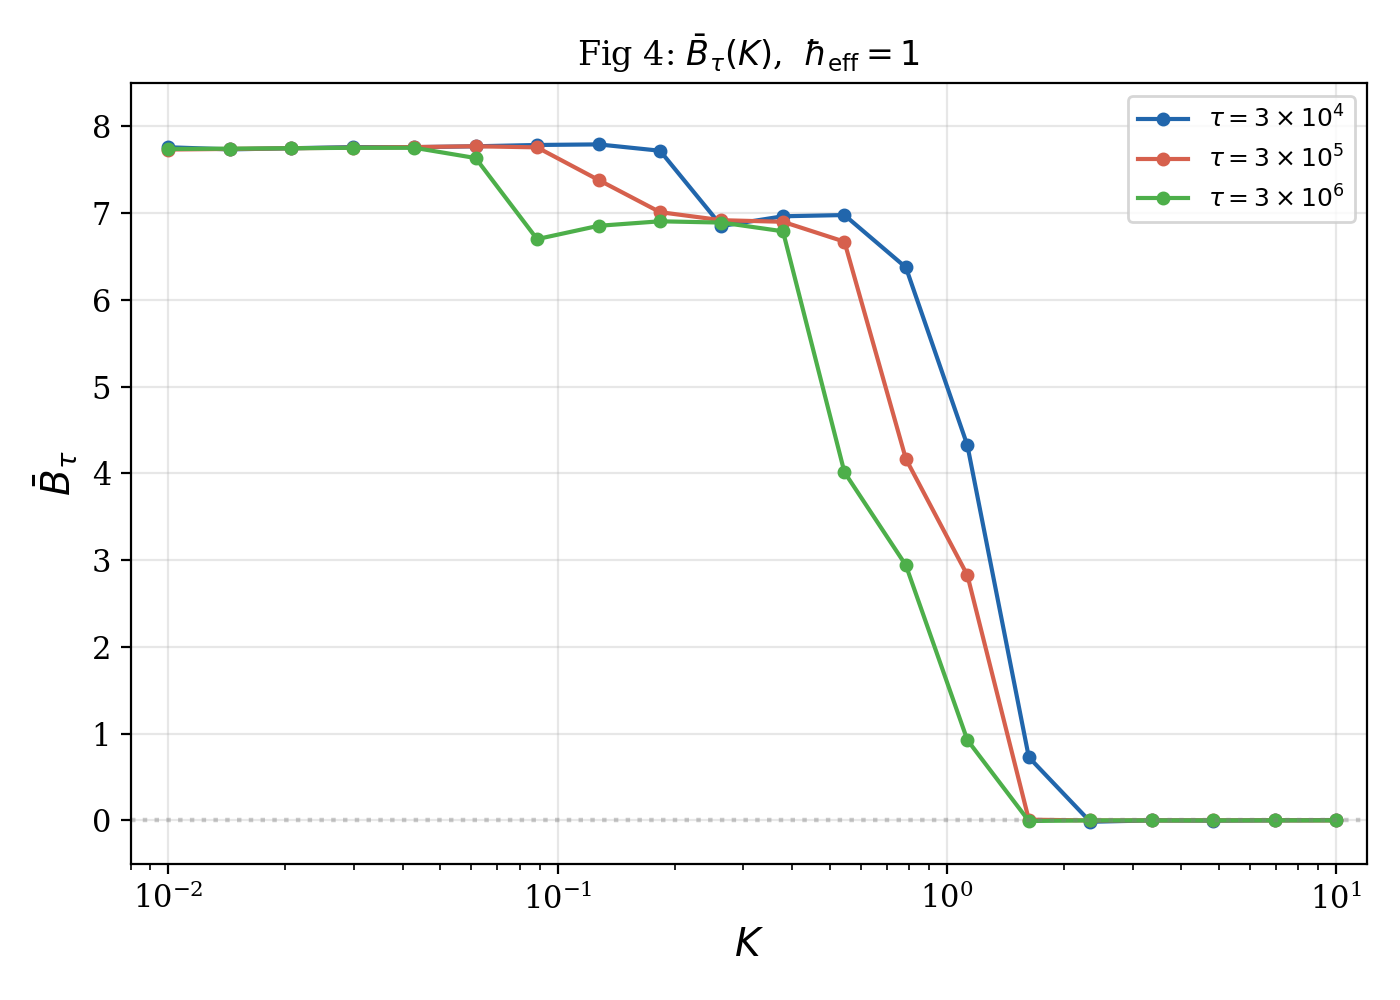
\includegraphics[width=0.82\textwidth]{fig4.pdf}
\caption{Fig.~4. $\bar{B}_{\tau}(K)$ for $\tau=3\times10^{4},3\times10^{5},3\times10^{6}$. $\hb=1$, $\sigma=4$.}
\label{fig:fig4}
\end{figure}

\subsection{Fig.~5 --- Classical LE in Polar Representation}

\textbf{Theory:} The classical LE $\lambda(x,p)$ at $K=1$ (just above $K_{\rm cr}$) reveals the mixed phase space: regular KAM islands ($\lambda\approx0$, blue) embedded in a chaotic sea ($\lambda>0$, yellow/green). The polar representation $(\theta=x,\;r=p+16)$ displays the torus topology. The two classical Gaussian peaks at $(x=0,p=0)$ and $(x=\pi,p=0)$ illustrate the initial phase-space distribution overlapping with both regular and chaotic regions.

\textbf{Method:} Classical tangent-map LE on a $200\times200$ grid with $p\in[-16,16]$, $x\in[0,2\pi)$, 400~kicks per point. Interpolated to polar coordinates via \texttt{RegularGridInterpolator}.

\begin{figure}[htbp]
\centering
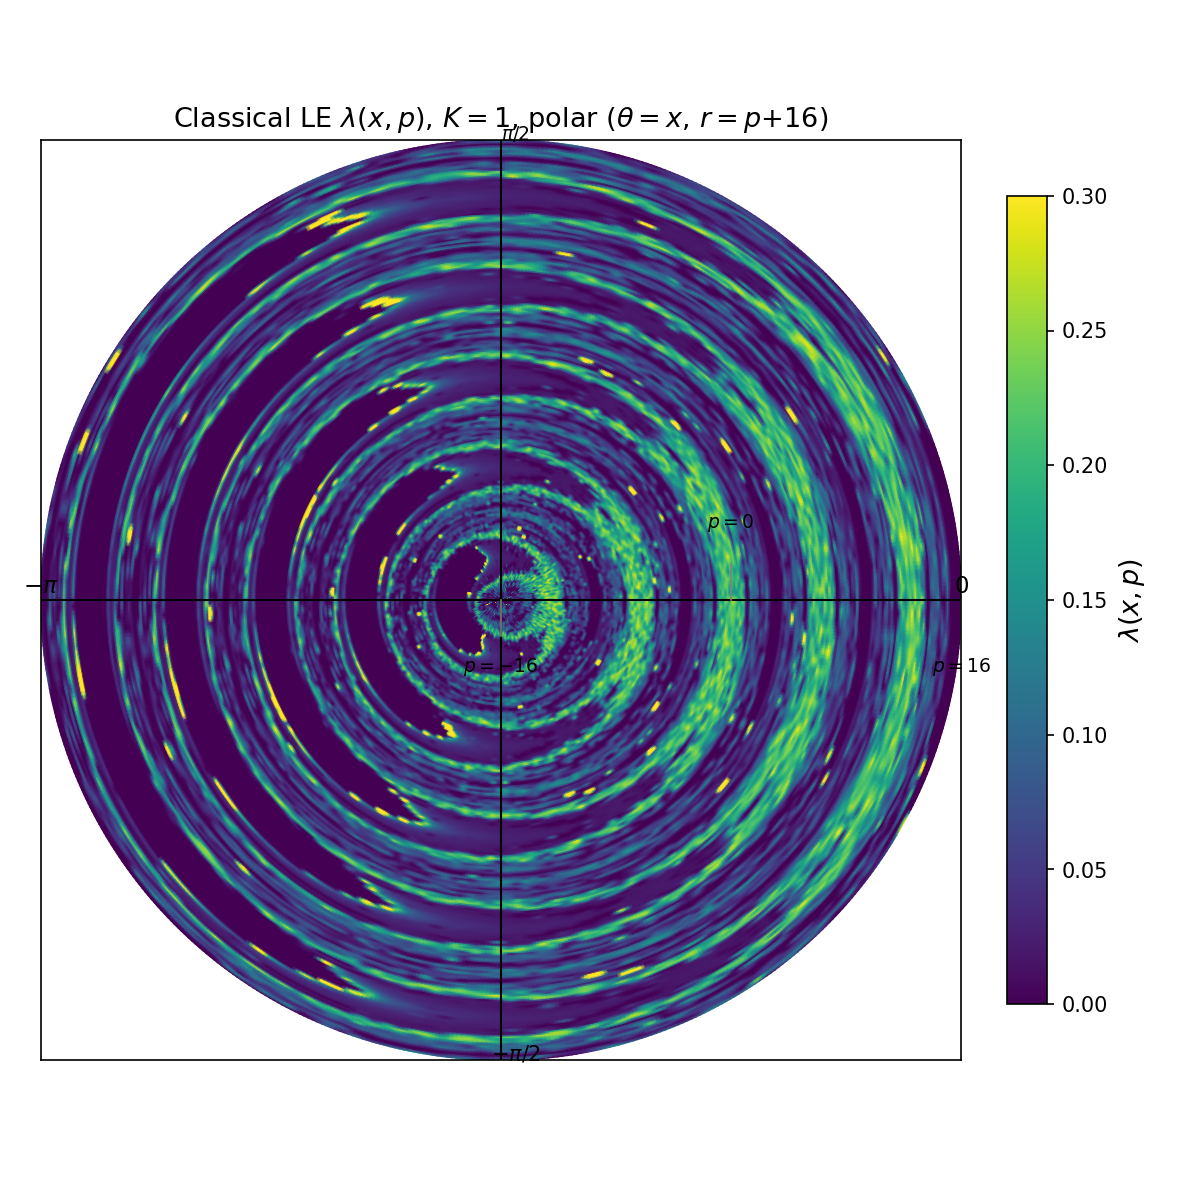
\includegraphics[width=0.72\textwidth]{fig5.png}
\caption{Fig.~5. Classical LE $\lambda(x,p)$ at $K=1$ in polar representation ($\theta=x$, $r=p+16$). Blue $=$ regular ($\lambda\approx0$), yellow $=$ chaotic ($\lambda\lesssim0.3$). The periodic concentric structure reveals the torus topology.}
\label{fig:fig5}
\end{figure}

%=============================================================================
\section{Computational Resource Assessment}
%=============================================================================

\subsection{Hardware}

\begin{itemize}[leftmargin=*]
\item \textbf{h100}: 2$\times$Intel Xeon Platinum 8558 (192 cores @ 2.1~GHz, hyperthreaded), 2~TB DDR5 RAM, 8$\times$NVIDIA H100 80~GB GPU.
\item \textbf{4090}: 2$\times$Intel Xeon Gold 5318Y (96 cores @ 2.1~GHz), 512~GB RAM.
\item \textbf{Storage}: Shared GPFS filesystem (\texttt{/gpfs/flash/home/}).
\item \textbf{Network}: h100 has no internet access; 4090 serves as the internet gateway for package installation.
\end{itemize}

\subsection{Per-Figure Resource Requirements}

\begin{table}[htbp]
\centering
\caption{Computational resources per figure. $\hb=2^{-14}$ unless noted.}
\label{tab:resources}
\begin{tabular}{@{}p{1.2cm}p{2.2cm}p{2cm}p{1.8cm}p{1.5cm}p{1.5cm}@{}}
\toprule
Figure & Method & Max.\ $N$ & Kicks & Wall Time & Memory \\
\midrule
Fig.~1 & Quantum Fwd--Bwd & $2^{21}$ & 30 & $\sim9$~min & $\sim4$~GB \\
Fig.~2 (classical) & Tangent-map MC & -- & 400 & $\sim18$~s & $<1$~GB \\
Fig.~2 (quantum) & Quantum Fwd--Bwd & $2^{23}$ & $5$--$12$ & $\sim2$~min & $\sim50$~GB \\
Fig.~3 ($K{=}3$) & Quantum Fwd--Bwd & $2^{20}$ & 100 & $\sim32$~min & $\sim2$~GB \\
Fig.~4 & Quantum Fwd-only & 32 & $3\times10^{6}$ & $\sim80$~s & $<1$~MB \\
Fig.~5 & Classical LE grid & -- & 400 & $\sim3$~min & $<1$~GB \\
\bottomrule
\end{tabular}
\end{table}

\subsection{Scaling Analysis}

\begin{itemize}[leftmargin=*]
\item \textbf{Fig.~1:} The $\mathcal{O}(T^{2})$ backward evolution dominates. For $T=30$, $\sim465$ backward steps per state type. For $T=100$, this grows to $\sim5050$ ($\sim11\times$).
\item \textbf{Fig.~2 quantum:} Basis $N=2^{23}$ ($8.4\times10^{6}$) for $K=1000$. FFT of size $2^{24}$ requires $\sim0.5$~s per transform. With $T=5$, total $\sim80$~FFTs.
\item \textbf{Fig.~4 scaling to $\tau=3\times10^{9}$:} The current FFT-based implementation achieves $\sim5\times10^{4}$~kicks/s at $N=16$. For $\tau=3\times10^{9}$, this would require $\sim17$~hours. A numba-accelerated implementation using precomputed $32\times32$ Floquet matrices is estimated at $\sim2\times10^{6}$~kicks/s, reducing the time to $\sim25$~min per $K$ value.
\item \textbf{Parallelism:} All figures parallelize over independent $K$ values and ensemble members via \texttt{multiprocessing.Pool}, with near-linear speedup up to the 192-core limit.
\end{itemize}

\subsection{Total Resource Footprint}

A complete reproduction of all five figures (excluding $\tau=3\times10^{9}$ in Fig.~4) requires approximately:
\begin{itemize}[leftmargin=*]
\item \textbf{CPU time:} $\sim45$~minutes (wall time, parallel execution)
\item \textbf{Peak memory:} $\sim50$~GB (Fig.~2 large-$K$ quantum tasks)
\item \textbf{Disk:} $<100$~MB for all data and figures
\end{itemize}

%=============================================================================
\section{Project Files}
%=============================================================================

\begin{itemize}[leftmargin=*]
\item \texttt{kicked\_rotor.py} --- Core library: standard map, tangent map, Floquet evolution, OTOC, Chirikov formula.
\item \texttt{run\_fig1.py / plot\_fig1.py} --- Quantum OTOC $C(t)$ and $B(t)$ (5~$K$, adaptive basis, ensemble avg).
\item \texttt{run\_fig2.py / plot\_fig2.py} --- Classical LE~+~CGR (80~$K$, grid~+~MC), Chirikov formula, inset.
\item \texttt{run\_fig2\_quantum.py} --- Quantum CGR extraction (29~$K$, adaptive kicks and basis).
\item \texttt{run\_fig2\_largeK.py} --- Large-$K$ quantum CGR ($K=200,500,1000$, $N$ up to $2^{26}$).
\item \texttt{run\_fig3.py / plot\_fig3.py} --- Logarithmic derivative $d(t)$ ($K=3,4,7,10$, 100~kicks).
\item \texttt{run\_fig4.py / plot\_fig4.py} --- Long-time averaged correlator ($\hb=1$, $N=16$, $\tau\leq3\times10^{6}$).
\item \texttt{run\_fig5.py} --- Classical LE in polar representation ($K=1$, $200\times200$ grid).
\item \texttt{fig1\_data.npz ... fig4\_data.npz} --- Raw numerical data.
\end{itemize}

\end{document}
